\subsection{Manipulasi Informasi pada Gerbang 1 Qubit}
Manipulasi informasi dalam arsitektur komputasi kuantum dilakukan secara esensial melalui penerapan berbagai gerbang logika yang direpresentasikan sebagai operator uniter U pada ruang vektor kompleks dua dimensi. Secara matematis, representasi matriks uniter paling umum untuk gerbang satu qubit diformulasikan melalui parameterisasi fisis yang melibatkan sudut rotasi θ dan tiga parameter fase kompleks independen yaitu $\alpha$, $\beta$, serta $\gamma$. Konfigurasi operasional dari parameterisasi matriks uniter tersebut dinyatakan ke dalam sebuah representasi persamaan matematis yang merepresentasikan transformasi kuantum umum
\begin{equation}
\label{eq:unitary_general}
U = e^{i\alpha} \begin{pmatrix} e^{i\beta}\cos\theta & e^{i\gamma}\sin\theta \\ -e^{-i\gamma}\sin\theta & e^{-i\beta}\cos\theta \end{pmatrix}.
\end{equation}
Penjabaran mengenai proses parameterisasi matriks uniter dua dimensi tersebut dari definisi awal hingga bentuk ekuivalen akhir disajikan secara komprehensif pada Lampiran \ref{app:penurunan_gerbang_uniter}. Melalui pemanfaatan bentuk matriks umum tersebut, observasi fisis terhadap berbagai macam gerbang uniter dasar kuantum dapat didemonstrasikan secara sistematis hanya dengan menyesuaikan konfigurasi parameter fase $\alpha$, $\beta$, $\gamma$, dan
sudut rotasi fisis $\theta$.

Matriks Pauli-X yang bertindak sebagai operator pembalik status keadaan $|0\rangle$ ke $|1\rangle$ dan sebaliknya, dapat diperoleh dengan menetapkan nilai sudut rotasi $\theta$ sebesar $\pi/2$. Pemilihan parameter sudut tersebut berimplikasi pada hilangnya kontribusi fungsi trigonometri kosinus dan menyisakan fungsi sinus bernilai satu pada elemen matriks. Untuk menyesuaikan elemen matriks agar bernilai satu, parameter fase relatif $\gamma$ dipilih sebesar $\pi/2$ sedangkan fase $\beta$ diatur bernilai nol. Dengan menetapkan nilai fase global $\alpha$ sebesar minus $\pi/2$, diperoleh matriks Pauli-X:
\begin{equation}
X = e^{-i\pi/2} \begin{pmatrix} 0 & e^{i\pi/2} \\ -e^{-i\pi/2} & 0 \end{pmatrix} = -i \begin{pmatrix} 0 & i \\ i & 0 \end{pmatrix} = \begin{pmatrix} 0 & 1 \\ 1 & 0 \end{pmatrix}.
\end{equation}
Matriks Pauli-Y juga dapat diperoleh dengan penyesuaian parameter sudut dan fase dari representasi uniter umum. Nilai sudut polar $\theta$ kembali dipilih sebesar $\pi/2$, sedangkan parameter fase relatif $\gamma$ diatur bernilai nol dan fase $\beta$ diatur bernilai nol. Penetapan nilai parameter tersebut menghasilkan bentuk matriks uniter yang didominasi oleh elemen bernilai riil pada bagian diagonal kedua matriks tersebut. Selanjutnya, dengan mengimplementasikan nilai fase global $\alpha$ sebesar $\pi/2$, diperoleh matriks Pauli-Y dengan penyimpangan fase global sebesar minus satu:
\begin{equation}
e^{i\pi/2} \begin{pmatrix} 0 & 1 \\ -1 & 0 \end{pmatrix} = i \begin{pmatrix} 0 & 1 \\ -1 & 0 \end{pmatrix} = \begin{pmatrix} 0 & i \\ -i & 0 \end{pmatrix} = -Y.
\end{equation}
Sementara itu, matriks Pauli-Z yang merepresentasikan pergeseran fase relatif pada keadaan qubit dapat diturunkan dengan menetapkan parameter sudut rotasi $\theta$ bernilai nol. Pemilihan nilai parameter sudut tersebut mengakibatkan elemen di luar diagonal utama bernilai nol karena kontribusi fungsi trigonometri sinus yang menghilang. Untuk memunculkan perbedaan tanda pada diagonal utama matriks, parameter fase relatif $\beta$ dipilih sebesar $\pi/2$ sedangkan fase $\gamma$ bernilai bebas. Selanjutnya, dengan mengalikan matriks tersebut dengan fase global $\alpha$ sebesar minus $\pi/2$, diperoleh representasi matriks Pauli-Z secara presisi tanpa adanya faktor fase imajiner tambahan:
\begin{equation}
Z = e^{-i\pi/2} \begin{pmatrix} e^{i\pi/2} & 0 \\ 0 & e^{-i\pi/2} \end{pmatrix} = -i \begin{pmatrix} i & 0 \\ 0 & -i \end{pmatrix} = \begin{pmatrix} 1 & 0 \\ 0 & -1 \end{pmatrix}.
\end{equation}
Langkah penyesuaian parameter fase ini secara konsisten membuktikan bahwa seluruh operator Pauli dasar merupakan representasi uniter dari grup khusus kuantum.

Matriks Pauli dapat dihimpun dan dinotasikan dengan $\sigma_x$, $\sigma_y$, dan $\sigma_z$ yang tetap merupakan operator Hermitian dan uniter dengan bentuk 
\begin{equation}
\label{eq:matriks_pauli}
\sigma_x = \begin{pmatrix} 0 & 1 \\ 1 & 0 \end{pmatrix}, \quad \sigma_y = \begin{pmatrix} 0 & -i \\ i & 0 \end{pmatrix}, \quad \text{dan} \quad \sigma_z = \begin{pmatrix} 1 & 0 \\ 0 & -1 \end{pmatrix}.
\end{equation}
Setiap representasi matriks Pauli tersebut difungsikan secara komputasional untuk memanipulasi informasi pada suatu \textit{qubit} tunggal melalui mekanisme pemetaan basis keadaan secara deterministik~\cite{fedorov_vqe_2022,hidalgo_quantum_2006}. Secara fungsional, gerbang Pauli-X setara dengan gerbang NOT pada sistem komputasi klasik, di mana status keadaan dari $|0\rangle$ ditukar menjadi $|1\rangle$ dan sebaliknya melalui operasi uniter tersebut. Secara aljabar, aksi pemetaan fisis dari operator Pauli-X terhadap himpunan basis komputasi tersebut dapat dinyatakan secara komprehensif melalui relasi kesamaan fisis berikut:
\begin{equation}
\label{eq:aksi_paulix}
X|0\rangle = |1\rangle, \quad X|1\rangle = |0\rangle.
\end{equation}
Di sisi lain, gerbang Pauli-Y melakukan pertukaran status keadaan komputasi sekaligus memberikan fase kompleks imajiner pada konfigurasi amplitudo probabilitas \textit{qubit}. Karakteristik operasional dari gerbang Pauli-Y tersebut secara geometris merepresentasikan rotasi fisis sebesar $180^\circ$ terhadap sumbu-y pada koordinat bola Bloch, yang aksi pemetaannya secara matematis dirumuskan sebagai:
\begin{equation}
\label{eq:aksi_pauliy}
Y|0\rangle = i|1\rangle, \quad Y|1\rangle = -i|0\rangle.
\end{equation}
Sementara itu, stabilitas nilai amplitudo probabilitas pada setiap basis komputasi dipertahankan secara teknis oleh gerbang Pauli-Z, tetapi tanda fase relatif antara keadaan $|0\rangle$ dan $|1\rangle$ dibalikkan oleh operator tersebut. Mekanisme pergeseran fase asimetris tersebut direpresentasikan dengan rotasi sebesar $180^\circ$ terhadap sumbu-z pada ruang Hilbert melalui pemetaan fisis:
\begin{equation}
\label{eq:aksi_pauliz}
Z|0\rangle = |0\rangle, \quad Z|1\rangle = -|1\rangle.
\end{equation}

Selain variasi gerbang Pauli, gerbang Hadamard ($H$) direpresentasikan sebagai gerbang logika satu \textit{qubit} yang  mana berasal dari pencarian vektor eigen dari gerbang Pauli-X. Pencarian vektor eigen tersebut diawali dengan persamaan untuk mencari nilai eigen $\lambda$ dari matriks Pauli-X yang beroperasi di dalam ruang Hilbert dua dimensi. Nilai eigen dari sebuah operator kuantum dapat diperoleh dengan menghitung nilai determinan dari selisih antara matriks Pauli-X dan perkalian skalar matriks identitas yang disamakan dengan nilai nol~\cite{kumar_family_2025,sim_expressibility_2019}. Pencarian himpunan nilai eigen tersebut dapat dirumuskan melalui persamaan
\begin{equation}
\label{eq:eigen_value_x}
\det(X - \lambda I) = \det \begin{pmatrix} -\lambda & 1 \\ 1 & -\lambda \end{pmatrix} = \lambda^2 - 1 = 0.
\end{equation}
Sehingga diperoleh dua buah nilai eigen, yaitu $\lambda_1 = 1$ dan $\lambda_2 = -1$.

Setelah seluruh nilai eigen berhasil diperoleh, masing-masing vektor eigen dievaluasi dengan mensubstitusikan nilai $\lambda$ kembali ke dalam persamaan nilai eigen. Hubungan amplitudo antara komponen basis keadaan atas dan komponen basis keadaan bawah dihasilkan dari persamaan untuk representasi nilai eigen pertama bernilai $\lambda_1 = 1$~\cite{cohen_portfolio_2020}. Vektor eigen pertama yang mewakili keadaan kuantum positif dapat diperoleh dari persamaan
\begin{equation}
\label{eq:eigen_vector_1}
|+\rangle = \frac{1}{\sqrt{2}} \begin{pmatrix} 1 \\ 1 \end{pmatrix} = \frac{|0\rangle + |1\rangle}{\sqrt{2}}.
\end{equation}
Di sisi lain, sistem persamaan linier mengharuskan amplitudo dari komponen basis yang memiliki tanda sebaliknya memiliki nilai eigen kedua bernilai $\lambda_2 = -1$. Dengan syarat normalisasi, vektor eigen kedua yang merepresentasikan keadaan kuantum negatif dapat diperoleh lewat persamaan
\begin{equation}
\label{eq:eigen_vector_2}
|-\rangle = \frac{1}{\sqrt{2}} \begin{pmatrix} 1 \\ -1 \end{pmatrix} = \frac{|0\rangle - |1\rangle}{\sqrt{2}}.
\end{equation}
Hasil kedua vektor eigen yang saling ortogonal ini digunakan sebagai landasan utama untuk mendefinisikan susunan elemen matriks transformasi basis pada arsitektur sistem komputasi kuantum.

Representasi matriks dari gerbang uniter Hadamard dapat dikonstruksi dengan menyusun kedua vektor eigen hasil dari operator Pauli-X tersebut sebagai komponen kolom~\cite{wang_achieving_2025,li_ising_2023,datta_relationship_2015}. Sebuah bentuk perkalian konstanta terhadap elemen matriks yang memiliki konfigurasi tanda asimetris dapat diperoleh lewat mekanisme penyusunan vektor eigen ortogonal ini dengan relasi matematis
\begin{equation}
\label{eq:matriks_hadamard}
H = \begin{pmatrix} |+\rangle & |-\rangle \end{pmatrix} = \frac{1}{\sqrt{2}} \begin{pmatrix} 1 & 1 \\ 1 & -1 \end{pmatrix}.
\end{equation}
Dari konstruksi matriks tersebut, basis komputasi gerbang Hadamard menunjukkan suatu kombinasi linier dari superposisi untuk memfasilitasi algoritma komputasi yang bersifat paralel. Oleh karena itu, operator Hadamard dapat dipetakan terhadap masing-masing basis ortogonal di dalam ruang Hilbert dua dimensi melalui hubungan
\begin{equation}
\label{eq:aksi_hadamard}
H|0\rangle = \frac{|0\rangle + |1\rangle}{\sqrt{2}}, \quad H|1\rangle = \frac{|0\rangle - |1\rangle}{\sqrt{2}}.
\end{equation}
Representasi skematis dari operasi matriks Pauli dan gerbang Hadamard tersebut dapat divisualisasikan pada Gambar \ref{fig:gerbang_pauli}, di mana kotak berlabel $X$, $Y$, $Z$, dan $H$ menunjukkan masing-masing gerbang logika kuantum dasar yang bekerja pada alur data qubit.
\begin{figure}[htbp]
    \centering
    \begin{tikzpicture}[scale=1.3, >=stealth]
        % Gerbang X
        \draw (0,1) -- (2,1);
        \draw[fill=white] (0.6,0.7) rectangle (1.4,1.3) node[midway] {$X$};
        
        % Gerbang Y
        \draw (3,1) -- (5,1);
        \draw[fill=white] (3.6,0.7) rectangle (4.4,1.3) node[midway] {$Y$};
        
        % Gerbang Z
        \draw (6,1) -- (8,1);
        \draw[fill=white] (6.6,0.7) rectangle (7.4,1.3) node[midway] {$Z$};
        
        % Gerbang H
        \draw (9,1) -- (11,1);
        \draw[fill=white] (9.6,0.7) rectangle (10.4,1.3) node[midway] {$H$};
    \end{tikzpicture}
    \caption{Simbolisme gerbang Pauli dan gerbang Hadamard pada sirkuit kuantum yang merepresentasikan transformasi uniter dasar $X$, $Y$, $Z$, dan $H$ pada satu \textit{qubit}.}
    \label{fig:gerbang_pauli}
\end{figure}

Matriks-matriks generator Pauli tersebut selanjutnya dapat digunakan sebagai basis operator untuk merepresentasikan arah rotasi dari vektor keadaan qubit pada koordinat bola Bloch~\cite{wang_variational_2025}. Setiap elemen dari grup khusus uniter $SU(2)$ dapat diekspresikan melalui kombinasi linier dari matriks Pauli:
\begin{equation}
U = e^{-i\frac{\theta}{2}(n_x X + n_y Y + n_z Z)} = e^{-i\frac{\theta}{2}(\hat{n}\cdot\vec{\sigma})},
\end{equation}
dengan $\vec{\sigma} = (X, Y, Z)$ merupakan vektor matriks Pauli dan $\hat{n} = (n_x, n_y, n_z)$ menyatakan parameter vektor satuan arah rotasi fisis. Evolusi uniter dari keadaan kuantum di bawah pengaruh generator Pauli tersebut dinyatakan dalam bentuk fungsi eksponensial dari operator proyeksi terkait $\hat{p} = \hat{n}\cdot\vec{\sigma}$. Menggunakan ekspansi deret Taylor dan pemisahan suku ganjil-genap dengan sifat $\hat{p}^2=I$, operator eksponensial tersebut dapat ditransformasikan menjadi bentuk identitas Euler kuantum melalui proses berikut:
\begin{equation}
\begin{split}
    e^{-i \frac{\theta}{2}\hat{p}} &= \sum_{n=0}^\infty \frac{(-i \frac{\theta}{2}\hat{p})^n}{n!} \\
    &= \sum_{k=0}^\infty \frac{(-i \frac{\theta}{2})^{2k} \hat{p}^{2k}}{(2k)!} + \sum_{k=0}^\infty \frac{(-i \frac{\theta}{2})^{2k+1} \hat{p}^{2k+1}}{(2k+1)!} \\
    &= \left( \sum_{k=0}^\infty \frac{(-1)^{k} (\frac{\theta}{2})^{2k}}{(2k)!} \right) I + \left( \sum_{k=0}^\infty \frac{(-1)^{k} (\frac{\theta}{2})^{2k+1}}{(2k+1)!} \right) \hat{p} \\
    &= \cos\left(\frac{\theta}{2}\right) I - i \sin\left(\frac{\theta}{2}\right) \hat{p}
\end{split}
\end{equation}

Dengan mensubstitusikan operator proyeksi arah $\hat{p}$ dengan masing-masing matriks generator Pauli ($\sigma_x$, $\sigma_y$, $\sigma_z$) ke dalam identitas Euler tersebut, diperoleh representasi matriks eksplisit untuk gerbang rotasi kuantum satu qubit sebagai berikut:
\begin{equation}
\label{eq:gerbang_rotasi_spesifik}
\begin{split}
    R_x(\theta) &= e^{-i \theta X/2} = \cos\frac{\theta}{2} I - i\sin\frac{\theta}{2} X = \begin{pmatrix} \cos\frac{\theta}{2} & -i\sin\frac{\theta}{2} \\ -i\sin\frac{\theta}{2} & \cos\frac{\theta}{2} \end{pmatrix},\\
    R_y(\theta) &= e^{-i \theta Y/2} = \cos\frac{\theta}{2} I - i\sin\frac{\theta}{2} Y = \begin{pmatrix} \cos\frac{\theta}{2} & -\sin\frac{\theta}{2} \\ \sin\frac{\theta}{2} & \cos\frac{\theta}{2} \end{pmatrix}, \\
    R_z(\theta) &= e^{-i \theta Z/2} = \cos\frac{\theta}{2} I - i\sin\frac{\theta}{2} Z = \begin{pmatrix} e^{-i\theta/2} & 0 \\ 0 & e^{i\theta/2} \end{pmatrix}.
\end{split}
\end{equation}
Ketersediaan parameter sudut rotasi $\theta$ ini menjadi landasan utama bagi algoritma optimasi klasik untuk mencari konfigurasi energi terendah pada lanskap Hamiltonian Ising yang sangat kompleks. Representasi skematik dari gerbang rotasi satu parameter tersebut divisualisasikan pada Gambar \ref{fig:gerbang_rotasi}, di mana kotak berlabel $R_x(\theta)$, $R_y(\theta)$, dan $R_z(\theta)$ menunjukkan masing-masing operasi transformasi uniter yang bekerja pada alur data qubit.
\begin{figure}[htbp]
    \centering
    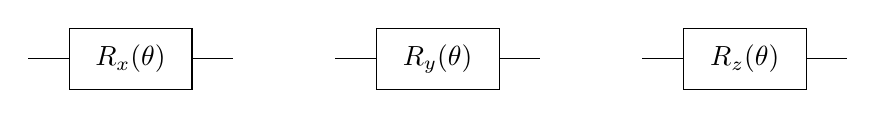
\begin{tikzpicture}[scale=1.3, >=stealth]
        % Gerbang R_x
        \draw (0,1) -- (2,1);
        \draw[fill=white] (0.4,0.7) rectangle (1.6,1.3) node[midway] {$R_x(\theta)$};
        
        % Gerbang R_y
        \draw (3,1) -- (5,1);
        \draw[fill=white] (3.4,0.7) rectangle (4.6,1.3) node[midway] {$R_y(\theta)$};
        
        % Gerbang R_z
        \draw (6,1) -- (8,1);
        \draw[fill=white] (6.4,0.7) rectangle (7.6,1.3) node[midway] {$R_z(\theta)$};
    \end{tikzpicture}
    \caption{Simbolisme gerbang rotasi pada sirkuit kuantum yang merepresentasikan rotasi parameter tunggal pada sumbu-X, sumbu-Y, dan sumbu-Z di bola Bloch.}
    \label{fig:gerbang_rotasi}
\end{figure}